% ********** Rozdział 1 **********
\setlength{\headheight}{14.49998pt}
\addtolength{\topmargin}{-2.49998pt}
\chapter{Podstawowe Założenia Sieci}
\section{Cel Projektu}
Celem projektu było zaprojektowanie topologii sieciowej dla firmy produkującej oprogramowanie, uwzględniając potrzeby i wymagania różnych działów oraz zapewniając wydajność, bezpieczeństwo i skalowalność sieci. Projekt miał na celu stworzenie nowoczesnej, elastycznej i bezpiecznej infrastruktury sieciowej, która umożliwi sprawne funkcjonowanie wszystkich działów firmy. 

\section{Struktura Sieci}
Sieć została zaprojektowana z myślą o separacji ruchu sieciowego, kontrolowaniu dostępu oraz zapewnieniu wysokiej dostępności i redundancji. Podstawowe założenia sieci obejmują segmentację za pomocą VLAN-ów, zastosowanie redundancji połączeń oraz wdrożenie różnych technologii sieciowych.

\subsection{Segmentacja Sieci za Pomocą VLAN-ów}
Segmentacja sieci została zrealizowana przy użyciu VLAN-ów (Virtual Local Area Network). Każdy dział w firmie, taki jak administracja, programiści, menedżerowie, ochrona, monitoring, serwery i goście, został przypisany do osobnego VLAN-u. Poniżej przedstawiono główne VLAN-y używane w sieci:
\begin{itemize}
    \item \textbf{VLAN 10 (Admins)}: VLAN przypisany do zarządu i administracji, gdzie znajdują się komputery i serwery FTP zarządu oraz administracji.
    \item \textbf{VLAN 20 (Programmers)}: VLAN dla programistów, obejmujący komputery programistów oraz serwery FTP i DHCP.
    \item \textbf{VLAN 30 (Managers)}: VLAN dla menedżerów projektów, gdzie znajdują się komputery, serwer FTP i DHCP.
    \item \textbf{VLAN 40 (Security)}: VLAN dla ochrony, obejmujący komputery ochrony.
    \item \textbf{VLAN 50 (Monitoring)}: VLAN dla monitoringu, obejmujący kamery, serwer monitoringu oraz czujniki.
    \item \textbf{VLAN 60 (Servers)}: VLAN dla serwerów deweloperskich oraz wspólnego serwera FTP.
    \item \textbf{VLAN 70 (Guests)}: VLAN dla sieci Wi-Fi dla gości na parterze.
    \item \textbf{VLAN 80 (Guests2)}: VLAN dla sieci Wi-Fi dla gości na piętrze.
    \item \textbf{VLAN 95 (Black Hole)}: VLAN dla nieużywanych portów (black hole).
\end{itemize}

\section{Opis Pomieszczeń i Urządzeń w Topologii Sieci}
Diagram sieciowy przedstawia szczegółowy układ pomieszczeń w budynku firmy oraz urządzenia sieciowe przypisane do każdego pomieszczenia.



\begin{figure}[ht]
    \centering
    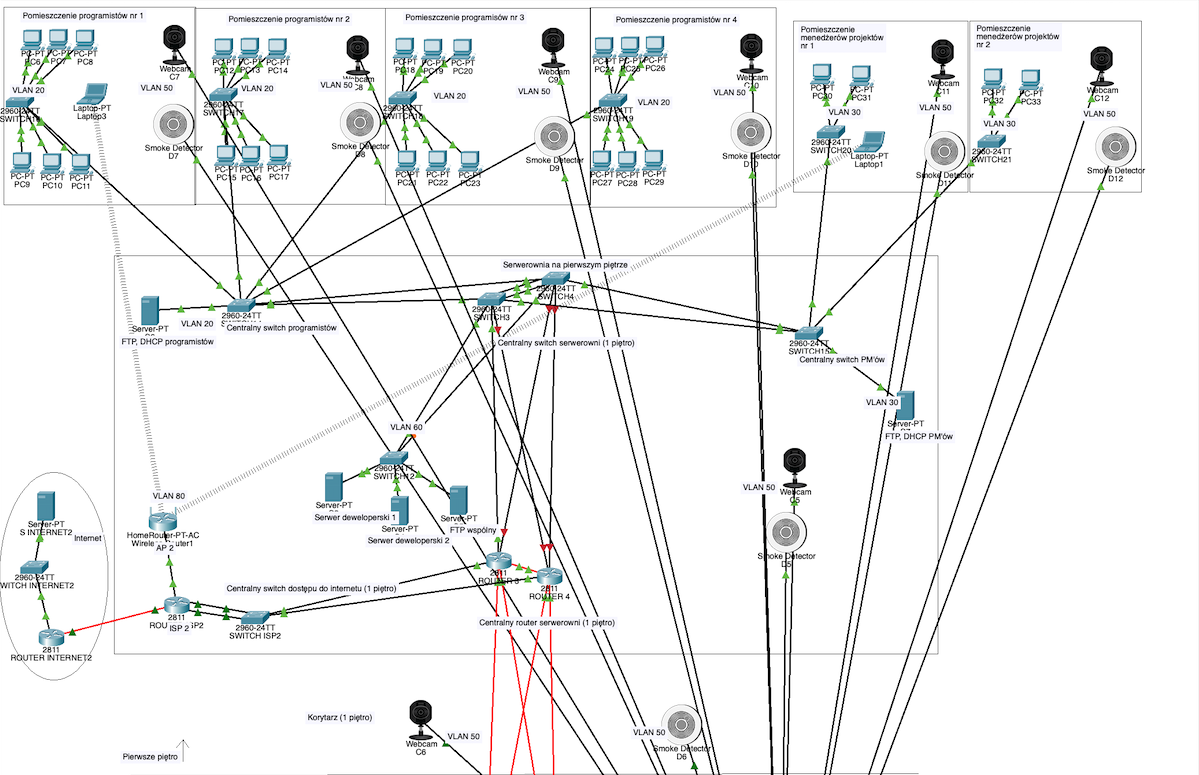
\includegraphics[width=0.8\textwidth]{Pietro.png}
    \caption{Diagram sieciowy - Pietro}
    \label{fig:pietro}
\end{figure}

\begin{figure}[ht]
    \centering
    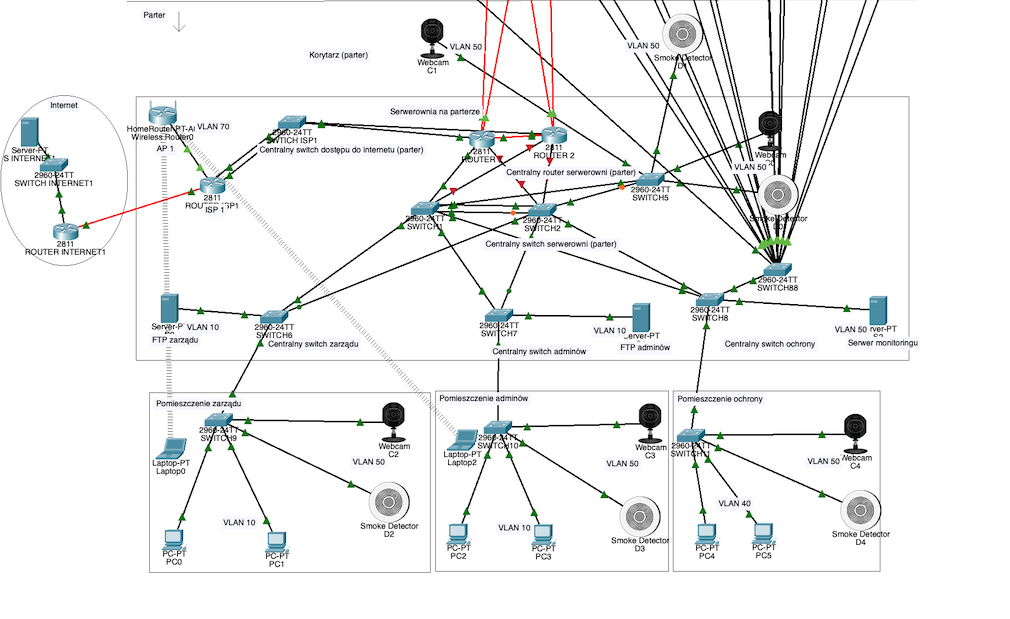
\includegraphics[width=0.8\textwidth]{Parter.png}
    \caption{Diagram sieciowy - Parter}
    \label{fig:parter}
\end{figure}

\newpage

\subsection{Pomieszczenia Programistów}
Pomieszczenia programistów są podzielone na cztery segmenty, z których każdy przypisany jest do VLAN 20. W każdym pomieszczeniu znajdują się komputery programistów oraz serwery FTP i DHCP. Dodatkowo, w każdym pomieszczeniu znajduje się smoke detector (czujnik dymu), co jest przykładem zastosowania urządzeń IoT (Internet of Things) do zwiększenia bezpieczeństwa w budynku.


\subsection{Pomieszczenie Menedżerów Projektów}
Pomieszczenie menedżerów projektów przypisane jest do VLAN 30. Znajdują się tam komputery menedżerów oraz serwery FTP i DHCP, które umożliwiają zarządzanie projektami i współpracę w ramach zespołu.

\subsection{Pomieszczenia Zarządu i Administracji}
Pomieszczenia zarządu i administracji są przypisane do VLAN 10. W tych pomieszczeniach znajdują się komputery i serwery FTP zarządu oraz administracji, co umożliwia zarządzanie firmą oraz administracyjne wsparcie dla innych działów.

\subsection{Pomieszczenia Ochrony}
Pomieszczenia ochrony są przypisane do VLAN 40. Znajdują się tam komputery ochrony oraz systemy monitoringu, które zapewniają bezpieczeństwo w budynku firmy.

\subsection{Pomieszczenia Monitoringu}
Pomieszczenia monitoringu przypisane są do VLAN 50. Znajdują się tam kamery monitoringu oraz serwery monitoringu, które rejestrują i przechowują dane wideo. W tych pomieszczeniach znajdują się również czujniki dymu, co jest kolejnym przykładem zastosowania urządzeń IoT.

\subsection{Serwerownia}
Serwerownia jest podzielona na dwa VLAN-y: VLAN 60 dla serwerów deweloperskich oraz VLAN 70 i VLAN 80 dla sieci Wi-Fi dla gości na parterze i piętrze. Serwerownia zawiera kluczowe serwery, takie jak serwery FTP i DHCP dla różnych działów oraz serwery deweloperskie, które wspierają pracę programistów.

\subsection{Korytarze i Strefy Wspólne}
W korytarzach i strefach wspólnych, takich jak pomieszczenia serwisowe, znajdują się przełączniki sieciowe oraz routery, które zapewniają łączność między różnymi segmentami sieci. Korytarze są również wyposażone w access pointy (AP) dla sieci Wi-Fi, które zapewniają bezprzewodowy dostęp do sieci dla gości.

\subsection{Zastosowanie Urządzeń IoT}
W całej topologii sieciowej zastosowano urządzenia IoT, takie jak kamery monitoringu i czujniki dymu. Kamery monitoringu są rozmieszczone w różnych pomieszczeniach i na korytarzach, zapewniając bezpieczeństwo i monitoring wizyjny. Czujniki dymu są zainstalowane w pomieszczeniach programistów oraz w pomieszczeniach monitoringu, co pozwala na szybkie wykrywanie pożarów i zwiększenie bezpieczeństwa w budynku.

\section{Hasła do Urządzeń Sieciowych}
W celu zapewnienia bezpieczeństwa sieciowego, każde urządzenie sieciowe zostało zabezpieczone hasłami. Poniżej znajduje się tabela z hasłami przypisanymi do poszczególnych urządzeń:

\begin{table}[!ht]
    \centering
    \caption{Hasła do Urządzeń Sieciowych}
    \begin{tabular}{|l|l|}
        \hline
        \textbf{Urządzenie} & \textbf{Hasło} \\ \hline
        Router1 & Router1 \\ \hline
        Router2 & Router2 \\ \hline
        Switch1 & Switch1 \\ \hline
        Switch2 & Switch2 \\ \hline
        Switch.ISP1 & Switch.ISP1 \\ \hline
        Switch5 & Switch5 \\ \hline
        Switch6 & Switch6 \\ \hline
        Switch7 & Switch7 \\ \hline
        Switch8 & Switch8 \\ \hline
        Switch88 & Switch88 \\ \hline
        Switch9 & Switch9 \\ \hline
        Switch10 & Switch10 \\ \hline
        Switch11 & Switch11 \\ \hline
        Router3 & Router3 \\ \hline
        Router4 & Router4 \\ \hline
        Switch3 & Switch3 \\ \hline
        Switch4 & Switch4 \\ \hline
        Switch.ISP2 & Switch.ISP2 \\ \hline
        Router.ISP2 & Router.ISP2 \\ \hline
        Switch12 & Switch12 \\ \hline
        Switch14 & Switch14 \\ \hline
        Switch15 & Switch15 \\ \hline
        Switch16 & Switch16 \\ \hline
        Switch17 & Switch17 \\ \hline
        Switch18 & Switch18 \\ \hline
        Switch19 & Switch19 \\ \hline
        Switch20 & Switch20 \\ \hline
        Switch21 & Switch21 \\ \hline
    \end{tabular}
\end{table}
\newpage
\section{SSID i Hasła do Sieci Wi-Fi}
Sieci Wi-Fi w firmie zostały skonfigurowane z odpowiednimi SSID i hasłami, zapewniając dostęp dla gości na różnych poziomach budynku.
\begin{itemize}
    \item \textbf{SSID: Parter, VLAN 70}
    \begin{itemize}
        \item Hasło: \textit{Parter!\@\#\$ (WPA2 Personal)}
    \end{itemize}
    \item \textbf{SSID: Pietro, VLAN 80}
    \begin{itemize}
        \item Hasło: \textit{Pietro!\@\#\$\% (WPA2 Personal)}
    \end{itemize}
\end{itemize}

\section{Podsumowanie}
Projekt topologii sieciowej dla firmy produkującej oprogramowanie uwzględniał różnorodne potrzeby działów firmy oraz zapewniał wysoką wydajność, bezpieczeństwo i skalowalność sieci. Dzięki segmentacji za pomocą VLAN-ów, redundancji połączeń oraz zastosowaniu nowoczesnych technologii sieciowych, sieć jest elastyczna, bezpieczna i gotowa na przyszłe rozwinięcia. Wdrożenie urządzeń IoT dodatkowo zwiększa bezpieczeństwo i funkcjonalność infrastruktury sieciowej.
